\newpage
\section{Background\label{introduction:background}}

\subsection{Breast Cancer Overview\label{sec:introduction:breastcanceroverview}}
Breast cancer is a type of cancer that starts in one or both breasts.

\subsubsection{Statistics\label{sec:introduction:breastcancer:statistics}}
Breast cancer accounts for about 30\% of all new cancer cases in U.S. women each year~\cite{RefWorks:RefID:150-2025breast}. The average risk of a woman in the U.S. developing breast cancer sometime in her life is about 1 in 8 (about 13\%)~\cite{RefWorks:RefID:36-american2021breast}. Breast cancer is also the second leading cause of cancer death in women behind lung cancer~\cite{RefWorks:RefID:36-american2021breast}.

\subsubsection{Development and Spread\label{sec:introduction:breastcancer:developmentandspread}}
Breast cancer can start in different parts of the breast, such as the ducts, lobules, or the tissue in between. The cancer can spread when cancer cells are carried to other parts of the body through blood or the lymphatic system. The lymphatic system is a network of small bean-sized glands called lymph nodes, ducts, and vessels that carry clear lymph fluid throughout the body. This clear lymph fluid contains immune system cells to fight infection as well as waste and tissue by-products. This system carries lymph fluid away from the breast; cancer cells can enter the lymph vessels, grow inside lymph nodes, and spread to other parts of the body~\cite{RefWorks:RefID:36-american2021breast}.

The most common areas where lymph vessels of the breast drain into are the underarm (axillary), inside the chest near the breastbone (internal mammary), and around the collar bone (supraclavicular and infraclavicular). Once cancer cells have spread to  the lymph nodes, there is a higher chance of metastases, or spreading, to other parts of the body which is called metastatic breast cancer~\cite{RefWorks:RefID:36-american2021breast}.

The method of cancer cells metastasizing through the lymphatic system is illustrated below in Figure~\ref{fig:introduction:lymphatic_system_in_a_breast} and Figure~\ref{fig:introduction:lymphatic_process_of_metastatic_breast_cancer}.

\begin{figure}[h!]
        \fbox{\begin{minipage}{0.92\textwidth}
                        \centering
                        \begin{subfigure}[b]{0.45\textwidth}
                                \centering
                                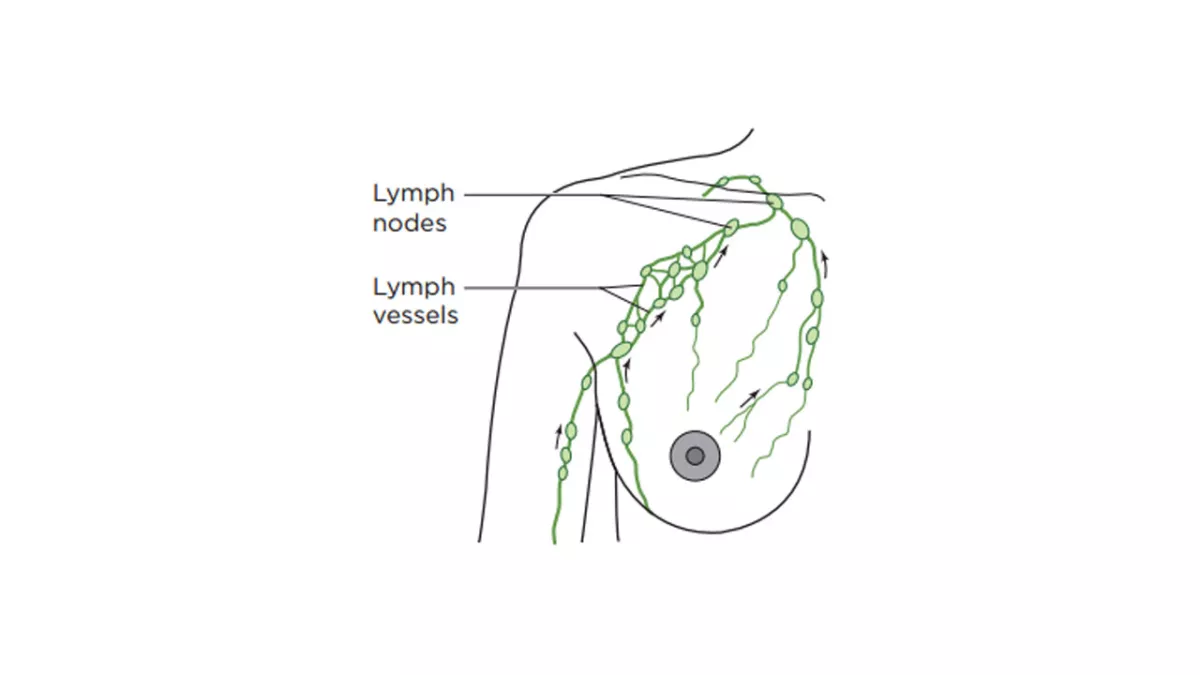
\includegraphics[width=\textwidth]{../figs/introduction/lymphatic_system_in_a_breast.png}
                                \caption{Lymphatic System Overview \cite{RefWorks:RefID:37-memorialsurgery}.}
                                \label{fig:introduction:lymphatic_system_in_a_breast}
                        \end{subfigure}
                        \begin{subfigure}[b]{0.45\textwidth}
                                \centering
                                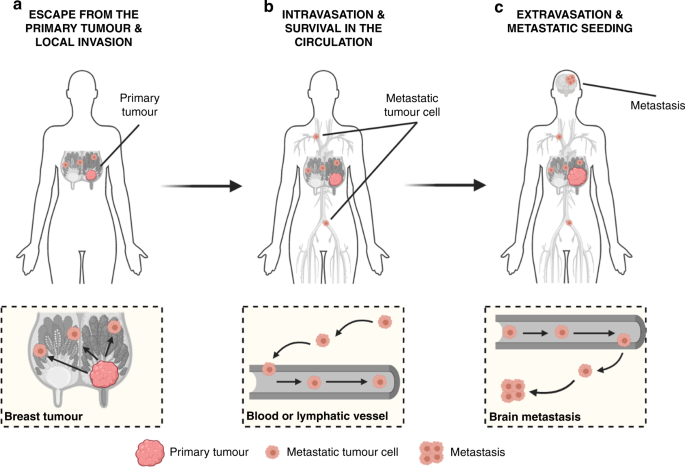
\includegraphics[width=\textwidth]{../figs/introduction/process_of_metastatic_breast_cancer.png}
                                \caption{Lymph Nodes Overview \cite{RefWorks:RefID:364-riggio2020lingering}.}
                                \label{fig:introduction:lymphatic_process_of_metastatic_breast_cancer}
                        \end{subfigure}
                \end{minipage}}
        \caption{Lymphatic System and Lymph Nodes Overview \cite{RefWorks:RefID:364-riggio2020lingering} \cite{RefWorks:RefID:37-memorialsurgery}.}
        \label{fig:introduction:lymphatic_system_and_nodes_overview}
\end{figure}

\subsection{Treatment of Breast Cancer\label{sec:introduction:treatmentofbreastcancer}}

\subsubsection{Stages of Breast Cancer\label{sec:introduction:breastcancer:stagesofbreastcancer}}
% Early vs late stage
Breast cancer is classified in stages ranging from 0 to IV based on the cancer's characteristics such as tumor size~\cite{RefWorks:RefID:151-2025breast}.

Stage 0 breast cancer is described as non-invasive, meaning the cancer cells are confined to the ducts or lobules in the breast and have not spread to surrounding healthy tissue~\cite{RefWorks:RefID:151-2025breast}.

Stage I breast cancer is invasive, meaning the cancer cells have spread to surrounding healthy tissue. In stage I breast cancer, the tumor is up to 2cm in size but invading cancer cells are no more than 1mm. Stage I is classified as either IA or IB depending on the sevarity of the cancer.~\cite{RefWorks:RefID:151-2025breast}.

Stage II breast cancer is used when the cancer is larger than 2cm but no larger than 5cm, or if the cancer has spread to one to three nearby lymph nodes. Similar to stage I breast cancer, stage II breast cancer can be subdivided into IIA and IIB~\cite{RefWorks:RefID:151-2025breast}.

Stage II breast cancer can be divided into IIIA, IIIB, and IIIC. This stage describes invasive breast cancer that is larger than 5cm or is found in four to nine nearby lymph nodes (IIIA), has spread to the chest wall or skin of the breast (IIIB), or has spread to ten or more nearby lymph nodes or to lymph nodes above or below the collarbone (IIIC)~\cite{RefWorks:RefID:151-2025breast}.

Lastly, stage IV breast cancer describes cancer that has metastasized, or spread, to other parts of the body such as the lungs, liver, bones, or brain~\cite{RefWorks:RefID:151-2025breast}.

Breast cancer stages can be divided into early and late stage breast cancer. Early-stage breast cancer incudes stages 0, I, and IIA while late-stage breast cancer includes stages IIB, III, and IV~\cite{RefWorks:RefID:365-stages}. Table~\ref{tab:introduction:breastcancer:stages} summarizes the stages of breast cancer. An overview of breast cancer treatment options for early and late stage breast cancer is shown in Figure~\ref{fig:introduction:breast_cancer_treatment_options_overview}.


\begin{table}[h!]
        \centering
        \caption{Stages of Breast Cancer~\cite{RefWorks:RefID:151-2025breast, RefWorks:RefID:365-stages}.}
        \label{tab:introduction:breastcancer:stages}
        \begin{tabular}{|c|c|c|}
                \hline
                \textbf{Stage} & \textbf{Description}                                       & \textbf{Early/Late Stage} \\
                \hline
                0              & Non-invasive, confined to ducts or lobules                 & Early                     \\
                \hline
                I              & Invasive, tumor up to 2cm, invading cells no more than 1mm & Early                     \\
                \hline
                IIA            & Tumor 2-5cm or spread to 1-3 lymph nodes                   & Early                     \\
                \hline
                IIB            & Tumor larger than 5cm or spread to 1-3 lymph nodes         & Late                      \\
                \hline
                IIIA           & Tumor larger than 5cm or found in 4-9 lymph nodes          & Late                      \\
                \hline
                IIIB           & Spread to chest wall or skin of breast                     & Late                      \\
                \hline
                IIIC           & Spread to 10+ lymph nodes or above/below collarbone        & Late                      \\
                \hline
                IV             & Metastasized to other parts of the body                    & Late                      \\
                \hline
        \end{tabular}
\end{table}

\subsubsection{Current Treatment Options\label{sec:introduction:breastcancer:currenttreatmentoptions}}

\subsubsection*{Surgical Options\label{sec:introduction:breastcancer:currenttreatmentoptions:surgicaloptions}}

Treatment options for breast cancer largely depend on the type and stage of the cancer. Surgical choices include a lumpectomy, which removes the tumor and a small margin of surrounding healthy tissue, or a mastectomy, which removes the entire breast~\cite{RefWorks:RefID:165-czajka2023breast}.

A lumpectomy is followed by radiation therapy to kill any stray cancer cells that may remain in the breast. This combination helps lower the risk of recurrence, or the return of the cancer~\cite{RefWorks:RefID:159-depolo2024radiation}. Radiation therapy is performed using high-energy X-rays to damage a cancer cell's DNA, preventing it from dividing further until it dies. Healthy tissue cells grow and divide slower than cancer cells, allowing them to repair themselves after radiation therapy while cancer cells cannot~\cite{RefWorks:RefID:159-depolo2024radiation}.

\subsubsection*{Lymph Node Biopsy\label{sec:introduction:breastcancer:currenttreatmentoptions:lymphnodebiopsy}}
In most surgical treatments for breast cancer, a lymph node biopsy is performed to check if cancer has spread past the breast tissue and to the lymph nodes. Samples from one or more lymph nodes are removed and examined under a microscope for cancer cells~\cite{RefWorks:RefID:37-memorialsurgery}. Standard practice was removing most of the lymph nodes in the underarm, called an axillary dissection. Today, a sentinel lymph node biopsy is more commonly performed to allow a faster recovery time~\cite{RefWorks:RefID:37-memorialsurgery}.

\subsubsection*{Sentinel Lymph Node Biopsy\label{sec:introduction:breastcancer:currenttreatmentoptions:sentinellymphnodebiopsy}}
The sentinel lymph node is the first lymph node that breast cancer cells spread to after leaving the breast. In a sentinel lymph node biopsy, a radioactive tracer (often technetium-99m) and/or a blue dye is injected into the side of the tumor. The tracer(s) travel through the lymphatic system to the sentinel lymph node. The blue stain and radiotracer signal, found with a gamma probe, can be used to identify and excise this lymph node for examination under a microscope for cancer cells~\cite{RefWorks:RefID:37-memorialsurgery},~\cite{RefWorks:RefID:165-czajka2023breast}.

\subsubsection*{Systemic Therapies\label{sec:introduction:breastcancer:currenttreatmentoptions:systemictherapies}}
While breast cancer treatment commonly starts with surgery, systemic therapies such as chemotherapy, hormone therapy, or targeted therapies may also be used~\cite{RefWorks:RefID:37-memorialsurgery}.

Chemotherapy, often called "chemo," uses strong medicines to slow or stop cancer cells from growing further. As chemotherapy often works by attacking cells that divide quickly, it can attack cancer cells but also other healthy cells that divide quickly such as those that make your hair grow. This can lead to side effects such as hair loss and nausea~\cite{RefWorks:RefID:37-memorialsurgery}.

Hormone treatment is used for breast cancer cells that require hormones such as estrogen to grow. This is done by blocking the hormones these cancer cells need to grow. Side effects can include changes in menstrual cycle, hot flashes, and aching bones~\cite{RefWorks:RefID:37-memorialsurgery}.

Targeted therapies, or precision medicines, attack specific characteristics of an individual's cancer cells rather than attacking all rapidly dividing cells like chemotherapy. Targeted therapies can treat the most common breast cancer gene mutations such as BRCA1 and BRCA2, HER2, and PIK3CA. This individualized treatment can lead to less side effects than in chemotherapy~\cite{RefWorks:RefID:37-memorialsurgery}.

\begin{figure}[h!]
        \centering
        \fbox{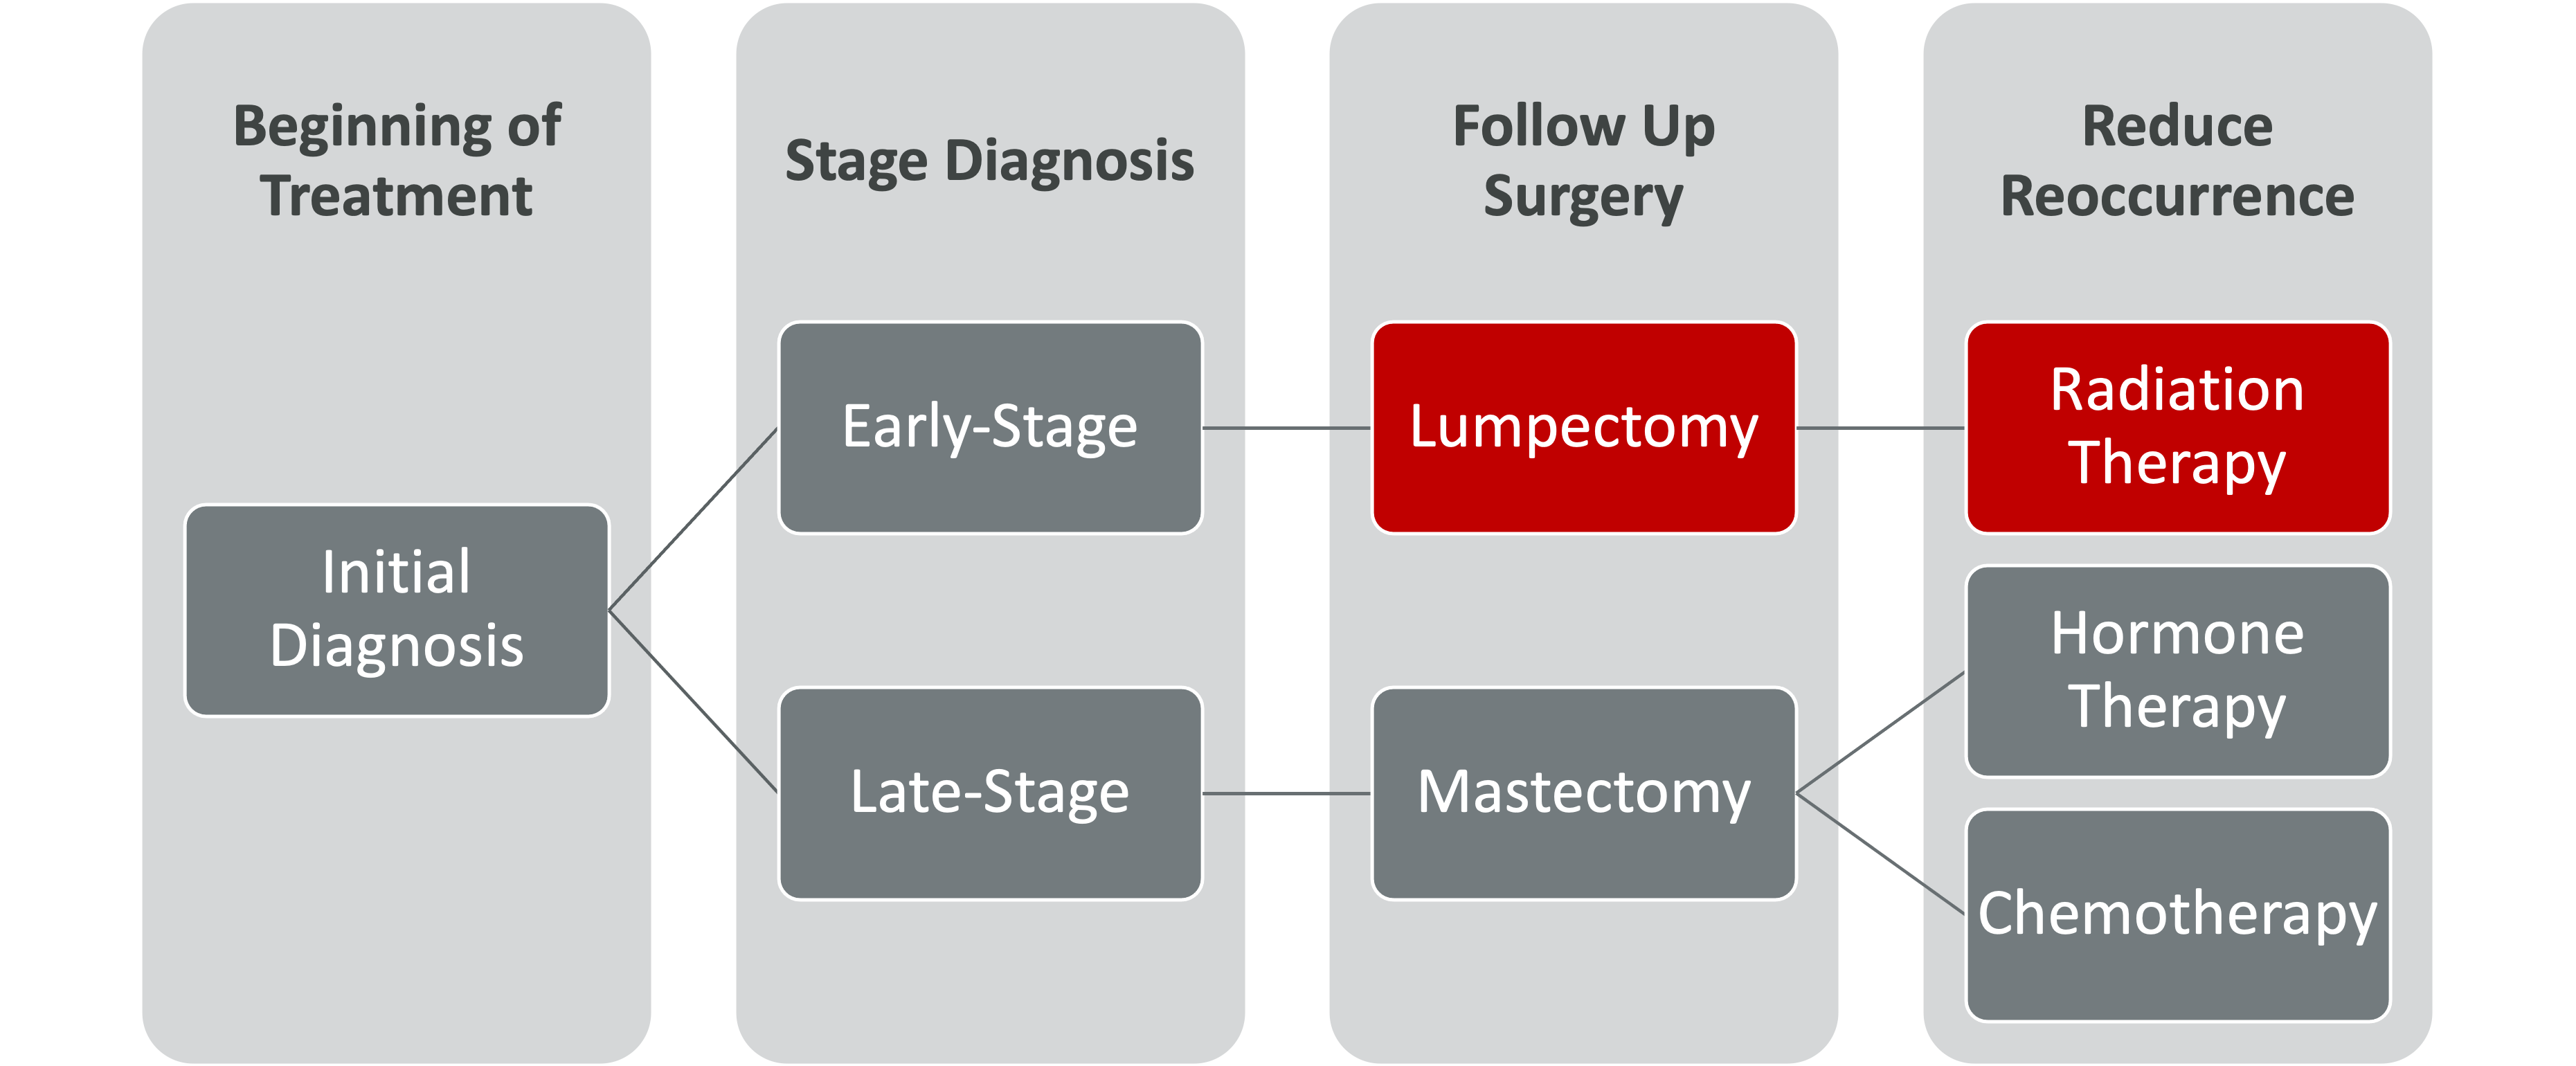
\includegraphics[width=0.6\textwidth]{../figs/introduction/breast_cancer_treatment_process_flowchart.png}}
        \caption{Breast Cancer Treatment Options Overview \cite{RefWorks:RefID:37-memorialsurgery}.}
        \label{fig:introduction:breast_cancer_treatment_options_overview}
\end{figure}

\newpage
\subsection{Motivation\label{sec:introduction:motivation}}
This is a subsection of the background in the introduction!
